\documentclass{article}

\author{A few good folks}

\title{Ahp coordination}
\usepackage[colorinlistoftodos]{todonotes}
\usepackage{graphicx}
\usepackage{mathtools}
\usepackage{times}
\usepackage{kpfonts}
\usepackage{subcaption}
\usepackage{multirow}
\usepackage{tabularx}
\usepackage{array}
\usepackage{algorithm}
\usepackage{algpseudocode}
\usepackage{tabularx}

\graphicspath{{./img/}}

% Naming conventions
% <fn><m><NAME>
% fn - prefix to distinguish newly-defined commands. Stands for "function"
% m - stands for "math". Indicates that it is used in the context of a $math expression$.

% Alternatives (nodes)
\newcommand{\fnmalts}{V_{N,1}, V_{N,2},\ldots}

% Aspects (nodes)
% arg 1 - indentifier of the level the nodes pertain to
\newcommand{\fnmasps}[1]{V_{#1,1}, V_{#1,2}, \ldots}

% Root node
\newcommand{\fnmroot}{V_{0,1}}

% Node
% arg 1 - level
% arg 2 - id
\newcommand{\fnmnode}[2]{V_{#1,#2}}

% Assessment in an aspect of a node, vector of weights
% arg 1 - level
% arg 2 - node (the aspect)
\newcommand{\fnmwasp}[2]{W_{#1}^{(#2)}}

% Indexed set of elements
% arg 1 - elements
% arg 2 - subscription index
\newcommand{\fnmsetind}[2]{\{ #1 \}_{#2}}

% Set of weights
% arg 1 - level for alternatives
% arg 2 - level for context
\newcommand{\fnmSetWasp}[2]{
    \fnmsetind
        % Content of  a set
        {\fnmwasp{#1}{\fnmnode{#2}{vert_{ #2 }}}}
        % Index
        {vert_{ #2 } \in L_{#2}}
}

% Short for for AHP
% arg1 - arg. #1 for AHP
% arg2 - arg. #2 for AHP
\newcommand{\fnmAhp}[2]{
    \mathbf{AHP}(#1, #2)
}

% Range
% arg 1 - from
% arg 2 - to
\newcommand{\fnmrange}[2]{\overline{#1, #2}}
% Naming conventions
% <fn><m|l><NAME>[Xi+]
% fn - prefix to distinguish newly-defined commands. Stands for "function"
% m - stands for "math". Indicates that it is used in the context of a $math expression$.
% l - stands for "listing"
% [Xi+] -  used to distinguish number of arguments for same commands which get overriden for number of arguments
%   For example, Xii stands for 2 arguments

% Alternatives (nodes)
\newcommand{\immodFnmalts}{V_{N,1}, V_{N,2},\ldots}

% Aspects (nodes)
% arg 1 - indentifier of the level the nodes pertain to
\newcommand{\immodFnmasps}[1]{V_{#1,1}, V_{#1,2}, \ldots}

% Root node
\newcommand{\immodFnmroot}{V_{0,1}}

% Node
% arg 1 - level
% arg 2 - id
\newcommand{\immodFnmnode}[2]{V_{#1,#2}}

% Assessment in an aspect of a node, vector of weights
% arg 1 - level, lower
% arg 2 - level, upper
% arg 3 - index, upper
\newcommand{\immodFnmwaspC}[3]{W_{#1}^{(\immodFnmnode{#2}{#3})}}

% Assessment in an aspect of a node, vector of weights
% arg 1 - level
% arg 2 - node (the aspect)
\newcommand{\immodFnmwasp}[2]{W_{#1}^{(#2)}}

% Indexed set of elements
% arg 1 - elements
% arg 2 - subscription index
\newcommand{\immodFnmsetind}[2]{\{ #1 \}_{#2}}

% Indexed set of elements
% arg 1 - elements
% arg 2 - subscription index
\newcommand{\immodFnmSetIndEbigg}[2]{\bigg\{ #1 \bigg\}_{#2}}

% Set of weights
% arg 1 - level for alternatives
% arg 2 - level for context
% arg 3 - index for the vertex at level #2
\newcommand{\immodFnmSetWaspC}[3]{ \immodFnmsetind{\immodFnmwasp{#1}{\immodFnmnode{#2}{#3}}}{#3 \in L_{#2}}}

% Set of weights
% arg 1 - level for alternatives
% arg 2 - level for context
\newcommand{\immodFnmSetWasp}[2]{\immodFnmSetWaspC{#1}{#2}{vert_{#2}}}

% Short for for AHP
% arg1 - arg. #1 for AHP
% arg2 - arg. #2 for AHP
\newcommand{\immodFnmAhp}[2]{
    \mathbf{AHP}(#1, #2)
}

% Range
% arg 1 - from
% arg 2 - to
\newcommand{\immodFnmrange}[2]{\overline{#1, #2}}

% Call a procedure
% arg 1 - procedure name
% arg 2 - arguments
\newcommand{\immodFnlCall}[2]{\textsc {#1} \big( #2 \big) }

% Form a set of AHP assessments in higher context for
%  the next recursive call
% arg1 - level, lower
% arg2 - level, intermediate
% arg3 - level, upper
% arg4 - index, intermediate
% arg5 - index, upper
\newcommand{\immodFnmAhpSet}[5] {
	\immodFnmSetIndEbigg
		{\immodFnlCall
			{AHP}
			{\immodFnmSetWaspC{#1}{#2}{#4}, \immodFnmwaspC{#2}{#3}{#5}}
		}
		{#5 \in L_{#3}}
}

% Tuple
\newcommand{\tuple}[1]{\left< #1 \right>}

% Nodes at level
 %arg 1 - level
\newcommand{\immodFnmNodesLvlB}[2]{\immodFnmsetind{\immodFnmnode {#1}{#2}}{#2 \in L_{#1}}}
\newcommand{\immodFnmNodesLvl}[1]{\immodFnmNodesLvlB{#1}{vert_{#1}}}


\begin{document}

    \maketitle

    \begin{abstract}
        Abstract
    \end{abstract}

    \section{Introduction}

    Multi agent systems and comlexity that goes along can be a source of a great excitement.
It is remarkable how a system comprising a set of agents with very limited capabilities to reasoning and decision making produces outstandingly good solutions to very difficult problems.
From global economy to simulated ant colonies, small agents applying their best "judgement" and acting in their own "interst" get things done.
It has been known for quite a long time that a beautiful whirl of a seemingly chaotic swarm of (semi-) independent agents is able to make solutions emerge.

But have we had solutions just appear by themselves, this world would not be half as spectacular.
The necessity to solve problems and the scarcity of low-hanging answers stimulate us to form structures and impose objectives on them, and as for multi agent ones we have two ways to go.
The first one is to set agents up and let them figure out a strategy through a series of interactions bearing significant information exchange.
As appealing as it is and as effective as it can be \cite{dorigo-2006}, we sometimes need something of a bigger certainty meaning that we want to express the objective in a more straightworward way.
The second one is to create a rigid system of absolute control.
When creating a PID controller for a UAV's stabilization algorithm, this is exactly what we want.
But for bigger and more complex systems, this approach may fall due to lack of flexibility.

The advantage of options in between those two extremes is arguably the flexibility those have. We can roughly delineate two
aspects in the process of that flexible group decision making: strategic and tactic. The first one pertains to
so-called "big picture". There exists some entity that is entitled to establish the direction of the group's strategy, given that it
has sufficient information, can reason in bigger-scale terms and define the general course of actions for the entire
group. However, it cannot (and should not) oversee all the details of the strategy's particular implementation
instances. It is better to delegate this part of decision making to smaller groups or individual agents. There is no
one-size-fits-all solutions in systems comprising multiple entities, and some decisions are better made in an ad-hoc
manner.
% TODO: "some" what?
Situational awareness \cite{endsley-1995} of individual agents may and often does possess detailed information that
is preferable to high-level instructions in the process of decision making.

In this paper, we propose an agent-based algorithm for load balancing in heterogenous networks that has two distinctive features.
First, it enables achieving load balance in a network of an arbitrary topology automatically, without any interventions on behalf of an entity maintaining the network, and regardless of the state the network is in by the moment the process of load balancing gets started.
Second, it allows separation of load balancing objectives into two levels: strategic and tactic.
This kind of separation loosens the influence of strategic objectives on  agents' (nodes) individual decision making, thus enabling the latter to handle local objectives in a more tailored fashion.




    % Tether to "load balancing" topic
% Reference the previous works: (1) Gorodetsky, load balancing, pass to a neighbour, (2) my paper w/ ahp



    \section{Generalized explaination of the approach}
    \label{sect:approachGen}

    %TODO: the fact that we we do not use tree structure violates "the lore". I have never seen AHP algorithms that would be
%implemented in this way.

%TODO: MAYBE: I have managed to formulate formal requirements for the graph that we use. What
%if I write them as well? I define there a notion of level (to some extent), and reveal constraints that make the
%recursive approach applicable.

%TODO: Constraints. We do not:
% 1. Delve into an agent's reasoning process;
% 2. Imply any particular structure of the graph;
% 3. Imply any particular implementation of an agent, neither its reasoning process (although we model that in our
%    "implementation" section)

% TODO: plan
% -- hierarchy of preferences
% ?? formal description of the graph. Definitions: levels
% -- separation of responsibilities, the actual approach to simulation
%TODO: Constraints. We do not:
    % 1. Delve into an agent's reasoning process;
    % 2. Imply any particular structure of the graph;
    % 3. Imply any particular implementation of an agent, neither its reasoning process (although we model that in our
    %    "implementation" section)
% -- definitions: aspects, contexts, levels
% -- fusion of tactical decisions up to the general objective (moving up the contexts)
% -- using AHP for this
% -- the recursive algorithm implementing the idea

In order to incorporate both strategic and tactical objectives into the decision making process we propose to represent
the latter as a result of decomposing strategic ones. By that, we do not necessarily mean that tactical objectives have
to be mutually exclusive components, represent dependencies or certain milestones, although that is definitely an
option. It implies that any lower-level objective may be a part of two or more higher-level ones. This decomposition can
be represented as a hierarchy of preferences or preference graph (Figure \ref{fig:prefgraph-concept-shared}).
%TODO: ref figure

\begin{figure}[hbt!]
    \centering
    \begin{subfigure}{.45\linewidth}
        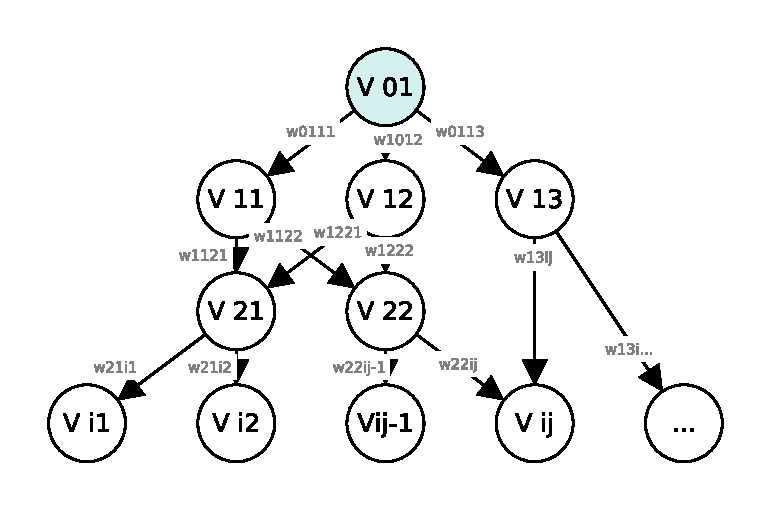
\includegraphics[width=\textwidth]{prefgraph-concept.eps}
        \caption{Shared graph}\label{fig:prefgraph-concept-shared}
    \end{subfigure}
    \begin{subfigure}{.45\linewidth}
        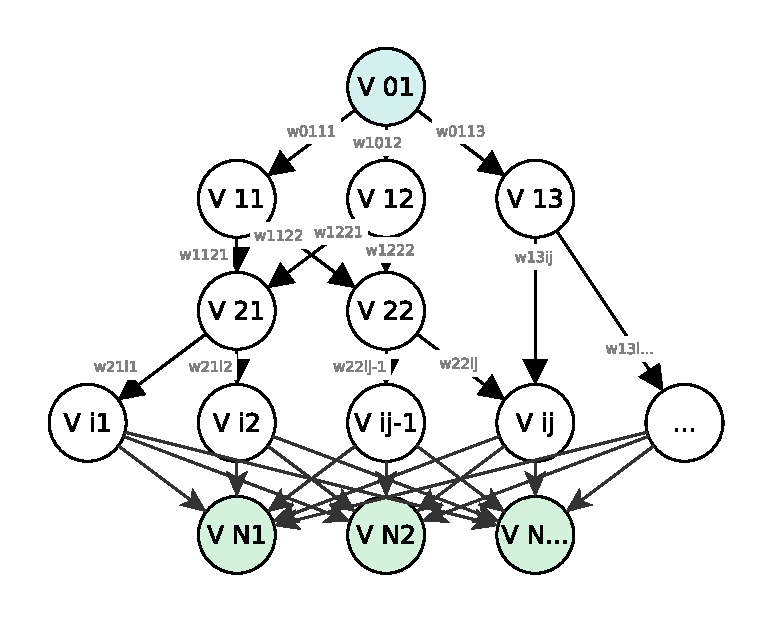
\includegraphics[width=\textwidth]{prefgraph-concept-extended.eps}
        \caption{Local graph}\label{fig:prefgraph-concept-local}
    \end{subfigure}

    \caption{\small An example of a preference graph}
    \label{fig:prefgraph-concept}
\end{figure}

However, this graph (Figure \ref{fig:prefgraph-concept-shared}) is only a part of a preference graph as it lacks
alternatives. Adding alternatives will give us a full-fledged preference graph (Figure
\ref{fig:prefgraph-concept-local}). For reasons that will soon become obvious we call graph in Figure
\ref{fig:prefgraph-concept-shared} "shared" and the one in Figure \ref{fig:prefgraph-concept-local} "local".

% To enrich
% the semantics of the decomposition process, we propose to not to limit it by just one iteration.


    \section{AHP-based algorithm for fusing strategic objectives into decision making}
    \label{sect:approachFormal}

    After the generic description and the main idea of the approach have been explained, let us suggest the algorithm for
assessing the alternatives $\fnmalts$ in the context of node $\fnmroot$. And we start with laying out some definitions,
constraints, and inputs most of which are intuitive but should be stated nonetheless.

\begin{itemize}
    % TODO: context
    \item Local graph is a weighted oriented graph;
    \item It has exactly one vertex without a parent (root); it also has vertices without children (alternatives);
    \item For any 2 edges $(a,b)$, $(a,c)$, there exist no paths between $b$ and $c$ (so the local
        graph can be divided into \textit{levels});
    \item A node's \textit{level} is the max. number of edges that should be traversed from the root $\fnmroot$ to
        achieve this node, or one of its peers;
    \item There exists a path to any alternative from any node (so we can gradually build the
        resulting vector level-by-level);
\end{itemize}

Here are notations used:

\begin{itemize}
    \item $\fnmnode i j$ denotes node $j$ of level $i$;
    \item $\fnmwasp k {\fnmnode i j}$ denotes a weights vector representing assessment of all nodes of level
        $k$ in the context of node $\fnmnode i j$;
    \item $L_i$ denotes an index set for nodes of level $i$.
\end{itemize}

As an input, we have a preference graph (local graph) $\left< V, E, W \right>$ ($V$ - nodes, $E$ - edges, $W$ - weights)
having $N$ levels. In the result, it is required to calculate $\fnmwasp N \fnmroot$ vector representing weights for
actions adjusted for strategic preferences, and assign an agent whatever action has the max. weight.


    \section{"Relay race" load balancing algorithm}

\cite{gorodetskii-2012} describes an approach to load balancing in a multi-agent network.
At first, a task gets passed to a randomly picked agent (node).
Each agent in the network implements the following decision-making algorithm.
It decides whether it should pass the task further to one of its neighbours, or hold it.
The decision is based on assessing the amount of tasks the agent's neighbours happen to run at the moment, in other words, how much they are loaded.
If there is no adjacent node with the amount of tasks less than that of the decision-making agent, the latter keeps the task.
Otherwise, it passes the task to its least loaded neighbour.
An experiment has shown that over time, tasks become uniformly distributed across the network.

However, this algorithm is not flexible enough, since it only enables optimizing against one objective.
There is a number of criterion that bear inportance to a network's performance, sustainability, and efficiency.
Moreover, the relative importance of those criterion to one another usually change over time.

%TODO: reference load balancing
%TODO: "our"
In our previous work \cite{murashov-2022}, we have devised an approach that combines AHP algorithm with the aforementioned "relay race".
A simulation has shown that the approach, indeed, enables on-demand fine tuning of the load balancing process without any direct intervention, while retaining all the advantages of the original algorithm.

However, the created model lacked separation of roles.
Agents could only use a pre-defined preference hierarchy graph without adjusting its weights, and make pass-or-keep decisions using a simple computational scheme.
Although this scheme is able to ensure that a network acquires the desired qualities of load distribution, or metrics of energy efficiency, pre-defined preferences still apply to the entire network.
Real world networks are highly dynamic, so it is not possible to devise a simple all-encompassing policy for each and every part of a cluster.
Some nodes appear, while other ones detach from the network.
So it would be helpful to have a model enabling high-level reasoning while leaving local decision making to individual agents (nodes).
% new node - load gap - old policy


In \cite{murashov-2022}, an agent would receive an input comprising preference hierarchy graph with pre-defined weights, the task itself, and meta-information regarding required technical capabilities a runner must possess.
Then it would compare its own state with that of its neighbours, assess those in the context of criterion used by the cluster, and make a pass-or-keep decision.
The set of those criterion consists of performance metric, energy efficiency, and load distribution uniformity.

Since the goal here is to achieve separation of local and global decision making, this preference hierarchy must be extended by additional levels.


    \label{sect:relayRace}

    \section{Conclusions}

The next generation of networks require formal foundations they reside upon to be able to handle high volatility of a network's topology.
Thus centralized control systems become more and more obsolete.
So we are glad to propose a solution that strikes the right balance between the necessity to control a system, the flexibility, and simplicity.

By this paper, we propose a new approach to solving load balancing problem through use of a combination of "relay race" and AHP algorithms.
The latter enables separation of strategic and tactic reasoning thus allowing the best-fit solutions to emerge, while the former, being indifferent to the topology of a system, takes care of its volatility aspect.
We also developed two extensible algorithm for both individual agents of a system (network nodes), and the coordinating entity that monitors the state of a network.


Here are the directions of this work's further development we would like to suggest.
The first one is creating an ontology of load balancing quality measures (or searching for an existing one that fits the purpose).
As we have stated before, the preference hierarchy we have proposed before (Figure \ref{fig:prefgraphLb}) only serves the immediate purpose of being an illustrative example.
Creating such an ontology would, in turn, enable creating a more generalized preference hierarchy graph.

Once an ontology is defined, finding good quality measures becomes the next step.
Our previous work \cite{murashov-2022} might serve as a starting point in this endeavour.
Some of measures used there might highlight some good solutions, on conceptual level at least.


    \label{sect:conclusion}

    \medskip

    \bibliographystyle{unsrt}

    \bibliography{bib}

\end{document}
